\section{Implementación}

\subsection{Ejercicio 1: Converger a una pose objetivo}

Para lograr la convergencia a la pose objetivo, la idea general será tomar el marco de referencia del objetivo como el marco inercial y desde ese nuevo marco calcular la posición del robot. Luego se irá acercando al objetivo.

Al acercarse al objetivo disminuye la distancia, y dado que la velocidad depende linealmente de la misma disminuye. Algo similar pasa con los angulos alfa y beta. Como puede verse en el siguiente gráfico al iniciar la trayectoria, se pondera mas el angulo alfa que respresenta un angulo entre el marco referencial del robot y el de la pose final. A medida que avanza pondera la dirección del angulo $\beta$ para llegar a la pose objetivo con el angulo deseado.

%%include graphics...
\begin{figure}[!h]
\begin{center}
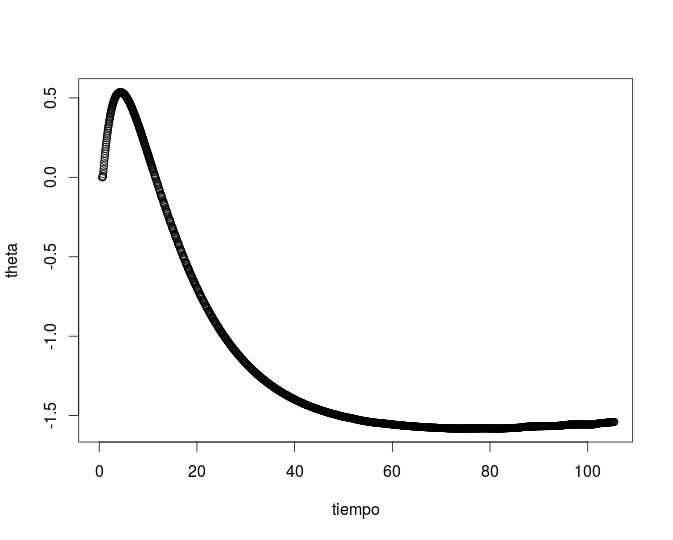
\includegraphics[scale=0.5]{ejercicio1}
\end{center}
\end{figure}
De esto se desprende que es importante que las constantes $K_\alpha$, $K_\beta$ y $K_\rho$ usadas tengan cierto equilibrio, para que el robot pueda alcanzar la pose adecuada con el angulo indicado. Por ejemplo un $K_\rho$ muy grande con valores pequeños de $K_\alpha$ y $K_\beta$ hará que el robot llegue en las coordenadas $x$ e $y$ pero con un angulo erroneo.Las tres constantes representan magnitudes, $K_\rho$ afecta de la velocidad lineal,$K_\alpha$ la dirección en que se gira para encarar el objetivo y el $K_\beta$ para alcanzar el angulo de la pose final.

\newpage

A partir de la experimentación con distintos valores, los siguientes valores resultaron adecuados:  %itemize c/ valores.

\begin{itemize}
\item $K_\alpha$:$0.1$
\item $K_\beta$:$0.25$
\item $K_\rho$:$-0.1$
\end{itemize}


A continuación graficamos la trayectoria del robot:

\begin{figure}[!h]
\begin{center}
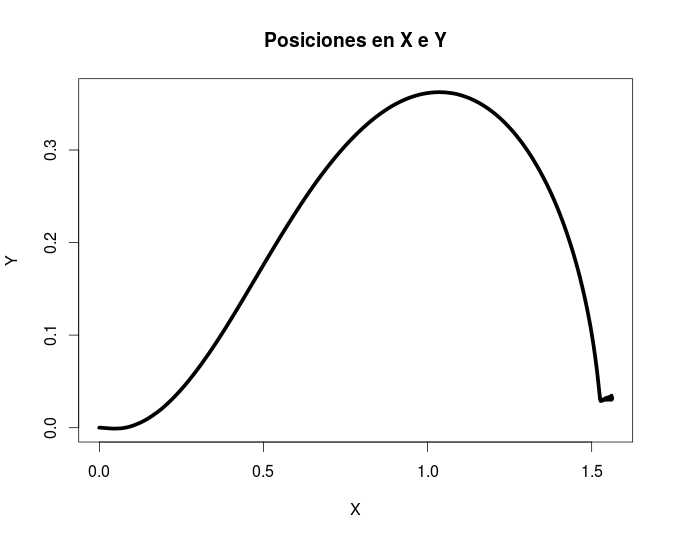
\includegraphics[scale=0.5]{ejercicio1b}
\end{center}
\end{figure}


En esta se puede observar que si bien el robot llega al objetivo, la trayectoria es poco controlable. Puede verse que comienza con mucha velocidad hacia el objetivo y a medida que se acerca disminuye de manera lineal hasta converger. Este tipo de control de trayectorias podria tener inconvenientes, ya que para un goal suficientemente alejado el robot comenzaría con velocidad excesiva, que podría no ser lo deseado.

\subsection{Ejercicio 2: Seguimiento de una trayectoria con requerimiento temporal}

Como ya introdujimos previamente, para esta sección, intentaremos restringir la posición del robot en base al tiempo.

Usando las constantes adecuadas en el modelo de pose de objetivo fija, lo que observamos fue que el robot no lograba cumplir con los requerimentos temporales definidos. Esto resulto ser así dado que las magnitudes K eran demasiado pequeñas, y el robot no alcanzaba la velocidad suficiente ni los angulos esperados.

Como solución a este problema tuvimos que agrandar las $K_\rho$ y $K_\alpha$, con el objetivo de lograr seguir fielmente la trayectoria esperada. Anulamos $K_\beta$ ya que en este ejercicio no requeriamos un angulo de entrada.

La trayectoria del robot respecto a la paso objetivo a medida que se avanzó fue la siguiente:

\begin{center}
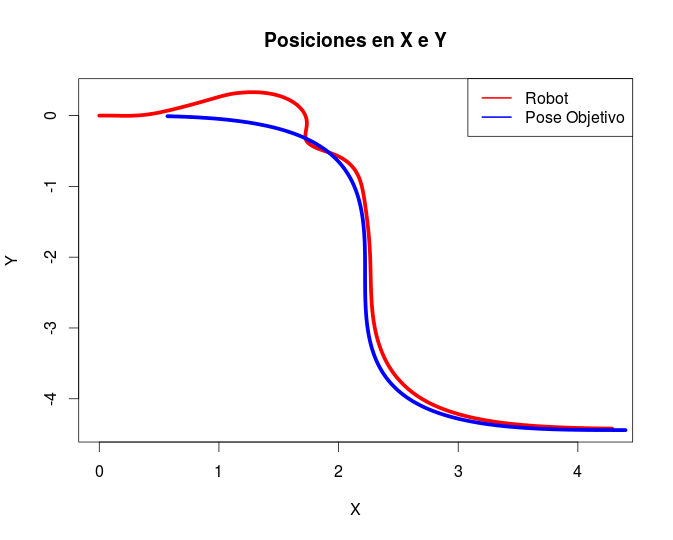
\includegraphics[scale=0.5]{ejercicio2}
\end{center}

En comparación con lo que ocurría en objetivo fijo la trayectoria es más suave.

Como desventaja de este sistema, podemos decir que estamos forzando al robot a mantener una velocidad a partir de requerimentos temporales que pueden ser realistas o no, de esta manera podriamos estar sobreexigiendolo o dandole poses poco realistas que el robot no pueda llegar a cumplir.

\subsection{Ejercicio 3: Algoritmo de seguimiento de persecucion}

Por último se plantea un algoritmo en el que se le entregan poses (waypoint) al robot para que este las cumpla. Una vez que este se encuentra a cierta distancia $lookahead$ de un waypoint, le asignamos uno nuevo a mayor distancia.

Utilizando los paramentros del apartado uno podemos observar que la trayectoria descripta sigue fielmente todos los waypoints establecidos.

%grafico
\begin{center}
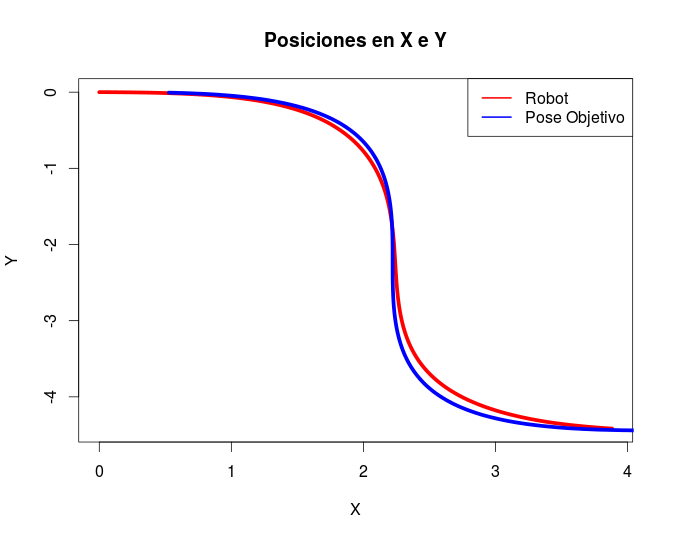
\includegraphics[scale=0.55]{ejercicio3c}
\end{center}

En cambio, utilizando los parametros del punto anterior podemos ver que se desprende bastante de la trayectoria original apenas comienza a aumentar su velocidad

%grafico
\begin{center}
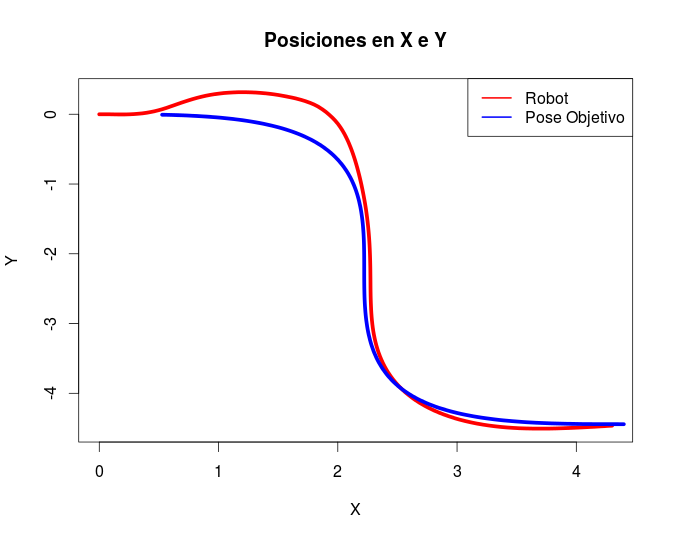
\includegraphics[scale=0.55]{ejercicio3b}
\end{center}

En comparacion con el modelo de requerimientos temporales, este algoritmo no es restrictivo con respecto al tiempo y solo debe recibir feedback del waypoint. Esto permite que el robot realice la trayectoria con una velocidad constante (con suficientes puntos, la distancia entre el robot y la pose siempre será mas o menos parecida) manteniendo la ventaja de poder describir una trayectoria más precisa.